%=====================================================================
\section{A harder problem -- a two-reservoir cascade}\label{sec:cascade}
%=====================================================================

The single reservoir turned out to be easy enough that a tuned
one-parameter rule matched PPO. Here the agent operates two reservoirs in
series. An uncontrolled tributary joins below them, so the agent must
coordinate where to hold flood space and when to release.

\subsection{System}
\begin{figure}[h]
\centering
\begin{tikzpicture}[>=Stealth, font=\small,
  res/.style={draw, thick, fill=blue!12, minimum width=2.4cm, minimum height=1.2cm, align=center}]
  \node[res] (A) at (0,0) {Reservoir A\\$S^A_{cap}=60{,}000$};
  \node[res] (B) at (6,0) {Reservoir B\\$S^B_{cap}=30{,}000$};
  \node[draw, thick, fill=blue!5, minimum width=2.4cm, minimum height=1.2cm, align=center] (F) at (12.4,0) {flood point\\$\Qsafe$, $D(t)$};
  \draw[->, very thick, blue!70] (0,1.8) node[above, font=\scriptsize]{$Q^A_{in}(t)$: large, slow catchment} -- (A.north);
  \draw[->, very thick, blue!70] (6,1.8) node[above, font=\scriptsize]{$Q^B_{in}(t)$: local catchment} -- (B.north);
  \draw[->, very thick, green!50!black] ([yshift=2mm]A.east) -- node[above, font=\scriptsize]{outlet A: $Q^A_t$ (agent)} ([yshift=2mm]B.west);
  \draw[->, thick, red!70] ([yshift=-3mm]A.east) -- node[below, font=\scriptsize]{spillway A} ([yshift=-3mm]B.west);
  \draw[->, very thick, green!50!black] ([yshift=2mm]B.east) -- node[above, font=\scriptsize]{outlet B: $Q^B_t$ (agent)} ([yshift=2mm]F.west);
  \draw[->, thick, red!70] ([yshift=-3mm]B.east) -- node[below, font=\scriptsize, pos=0.3]{spillway B} ([yshift=-3mm]F.west);
  \draw[->, very thick, orange!80!black] (10.4,-1.9) node[below, font=\scriptsize, align=center]{tributary $Q^{tr}(t)$\\(flashy, uncontrolled)} -- (10.4,-0.3);
\end{tikzpicture}
\caption{The two-reservoir cascade. Reservoir A's outflow, through its
outlet or spillway, enters reservoir B. The flood point and the downstream
users sit below the tributary confluence.}
\label{fig:cascade_schematic}
\end{figure}

Storms are regional: every storm hits all three catchments, with each
catchment responding at its own scale and speed (all flows in m$^3$/d):
\begin{center}
\small
\begin{tabular}{lrrrrr}
\toprule
catchment & base flow & peak scale $\bar P$ & delay & rise time & recession $k$ [d$^{-1}$] \\
\midrule
A (upstream, large) & 500 & 5{,}000 & 0.5 d & 1.0 d & $U(0.2,0.4)$\\
B (local) & 200 & 3{,}000 & 0 & 0.5 d & $U(0.4,0.7)$\\
tributary & 300 & 4{,}000 & 0 & 0.25 d & $U(0.7,1.2)$\\
\bottomrule
\end{tabular}
\end{center}
Storm onsets arrive with probability 0.05 per day. Each storm has a common
intensity $m\sim U(0.5,1.5)$, and catchment $c$ gets peak
$\bar P_c\,m\,U(0.8,1.2)$ with the hydrograph shape of
Section~\ref{sec:objective}. All base flows share one factor
$\beta\sim U(0.7,1.3)$. The demand at the flood point has mean
$\bar D=2{,}000$~m$^3$/d with a $\pm30\%$ seasonal swing. The river's safe
capacity is $\Qsafe=4{,}000$~m$^3$/d. The outlet capacities are
$Q^A_{\mathrm{out}}=6{,}000$ and $Q^B_{\mathrm{out}}=8{,}000$~m$^3$/d.

\paragraph{Calibrating the storm climate.} The first parameter set (storm
probability 0.07, peak scales 7{,}000/4{,}000/6{,}000) was too wet. Mean
inflow was about 314{,}000~m$^3$ per season, against about 280{,}000~m$^3$
the river can carry below $\Qsafe$ after the tributary. Even a rule that
releases at the safe limit every day spilled more than 100{,}000~m$^3$, so
penalties were dominated by unavoidable floods. With the values above, the
mean inflow is about 200{,}000~m$^3$ (A+B) plus 53{,}000~m$^3$ (tributary).
All three penalty types then matter, and the rule thresholds trade supply
against flooding (Figure~\ref{fig:cascade_tuning}).

\subsection{OHQ model}
Per decision step, the backend (\code{CascadeBackend}) builds two
\code{Reservoir} blocks and two \code{fixed\_head} sinks
(\code{River}, \code{SpillSinkB}), plus four \code{Reservoir\_link\_rule}
links: \code{outletA} and \code{spillwayA} (A$\to$B), \code{outletB}
(B$\to$\code{River}) and \code{spillwayB} (B$\to$\code{SpillSinkB}). They use
the same outlet and spillway parametrization as Section~\ref{sec:ohqmodel}.
B's released and spilled volumes come from the sink storages, as before.
A's outflow enters B rather than a sink, so its volumes are recovered from
A's storage at the end of every solver step. OHQ's time integration is
backward Euler, so the volume through a link over a step of length
$\Delta t_0$ is $Q(S_{\text{end of step}})\,\Delta t_0$:
\[
V^{rel,A}_t=\sum_{n}Q_{\text{outlet}}\big(S^A_n\big)\,\Delta t_0,\qquad
V^{sp,A}_t=\sum_{n}Q_{\text{spillway}}\big(S^A_n\big)\,\Delta t_0 .
\]
\textbf{Check.} B's mass balance, which includes these recovered A volumes
as inflow, closes over a season to within 0.5~m$^3$ of
$\sim$200{,}000~m$^3$ inflow. A's own balance closes to within 17~m$^3$.
Daily residuals of $\pm$100--200~m$^3$ on storm days are the same
inflow-sampling effect as in Figure~\ref{fig:massbalance}, and they cancel.
One cascade step costs about 10~ms.

\subsection{MDP and objective}
\begin{description}\itemsep2pt
\item[Observation] (16): $S^A_t/S^A_{cap}$, $S^B_t/S^B_{cap}$; the current
inflows of A, B and the tributary; noisy 1-, 2- and 3-day forecasts of the
daily-mean inflow of each of the three streams (9 values, same error
model as before); $D_t$; and $1-t/T$. Flows are divided by $\Qsafe$.
\item[Action] (2): $a_t\in[-1,1]^2$, mapped to
$Q^A_t=\tfrac12(a_{t,1}+1)Q^A_{\mathrm{out}}$ and
$Q^B_t=\tfrac12(a_{t,2}+1)Q^B_{\mathrm{out}}$.
\item[Reward:] with river flow at the flood point
$V^{riv}_t=V^{rel,B}_t+V^{sp,B}_t+V^{tr}_t$ (all over day $t$; $V^{tr}_t$
is the tributary volume),
\[
r_t=-\Big(\frac{\max(0,D_t-V^{riv}_t)}{D_t}\Big)^2
-w_f\frac{\max(0,V^{riv}_t-\Qsafe)}{\Qsafe}
-w_s\frac{V^{sp,A}_t+V^{sp,B}_t}{\Qsafe},
\]
plus the terminal term
$-\tfrac{w_T}{2}\big[\max(0,\tfrac12S^A_{cap}-S^A_T)/S^A_{cap}+\max(0,\tfrac12S^B_{cap}-S^B_T)/S^B_{cap}\big]$,
with the same weights as before.
\end{description}
The objective is again the expected undiscounted season return
$J(\pi)=\mathbb E_\xi\big[\sum_t r_t+r^{\mathrm{term}}_T\big]$,
Eq.~\eqref{eq:objective}.

\subsection{Baseline: a coordinated two-threshold rule}
The rule has thresholds $\eta_A,\eta_B$ (fractions of each capacity) and
uses the current tributary flow $q^{tr}_t$ and B's current inflow $q^B_t$
(both m$^3$/d). With $\Delta t=1$~d the drawdown time of excess storage,
Write the storage above each threshold as a flow by spreading it over one
day, and B's spare room per day:
\begin{align*}
E_A &= \frac{S^A_t-\eta_A S^A_{cap}}{\Delta t},\qquad
E_B = \frac{S^B_t-\eta_B S^B_{cap}}{\Delta t},\qquad
R_B = \max(0,-E_B)+Q^B_t-q^B_t \quad\text{(all m$^3$/d)}.
\end{align*}
Then
\begin{align*}
Q^{sup}_t &= \max(0,\,D_t-q^{tr}_t),\\
Q^B_t &= \begin{cases} \max\!\big(Q^{sup}_t,\ \min(\Qsafe-q^{tr}_t,\ Q^{sup}_t+E_B)\big) & E_B>0\\
Q^{sup}_t & E_B\le0,\end{cases}\\
Q^A_t &= \mathbf{1}[E_B<0]\,\max(0,\,Q^{sup}_t-q^B_t)\;+\;\mathbf{1}[E_A>0]\,\min\big(E_A,\ \max(0,R_B)\big).
\end{align*}
In words: $Q^{sup}_t$ is the part of the demand the tributary does not
supply. B releases it, plus its excess storage as far as the river capacity
left by the tributary allows. A keeps B supplied while B is below its
target, and releases its own excess as far as B has room for it.
both clipped to the outlet capacities. A first version backfilled
\emph{everything} B released, including flood releases, from A. That kept B
full, and the rule spilled about 90{,}000~m$^3$ per season regardless of
its thresholds. With the backfill restricted as above, the rule behaves
sensibly. ``Supply only'' is this rule with $\eta_A=\eta_B=1$ (never
release for flood space). The tuned rule's thresholds are chosen by grid
search over $\{0.1,\dots,0.9\}^2$ on 30 tuning seasons.

\begin{figure}[h]
\centering
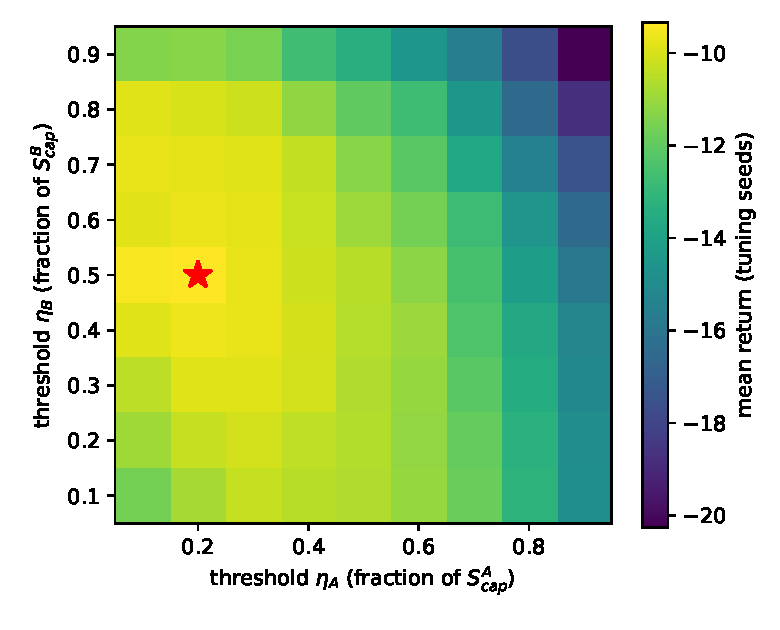
\includegraphics[width=0.55\textwidth]{figures/cascade_threshold_tuning.pdf}
\caption{Mean return of the cascade rule over its two thresholds (tuning
seasons). The star marks the tuned rule.}
\label{fig:cascade_tuning}
\end{figure}

\subsection{Training}
PPO uses the same networks and hyperparameters as in Section~\ref{sec:ppo},
with 16 inputs and two action dimensions, for about $10^6$ environment
steps with 16 workers (about 670 steps/s).
Training took about 28 minutes, about $10^6$ simulated days or 11{,}000
seasons, each day a full OHQ run of the two-reservoir model.
Figure~\ref{fig:cascade_learning} shows the return rising from about $-44$
(an untrained, essentially random policy) to about $-11$ after 160{,}000
steps, and to the $-4$ to $-9$ range after 500{,}000 steps. The curve stays
jagged because it averages only the last 20 training seasons, and those
seasons differ in storminess (and are run with exploration noise on). The
exploration spread $\sigma$ falls steadily from 0.59 to 0.18. The agent
becomes more confident but still explores, so more training might still
help a little.


\begin{figure}[h]
\centering
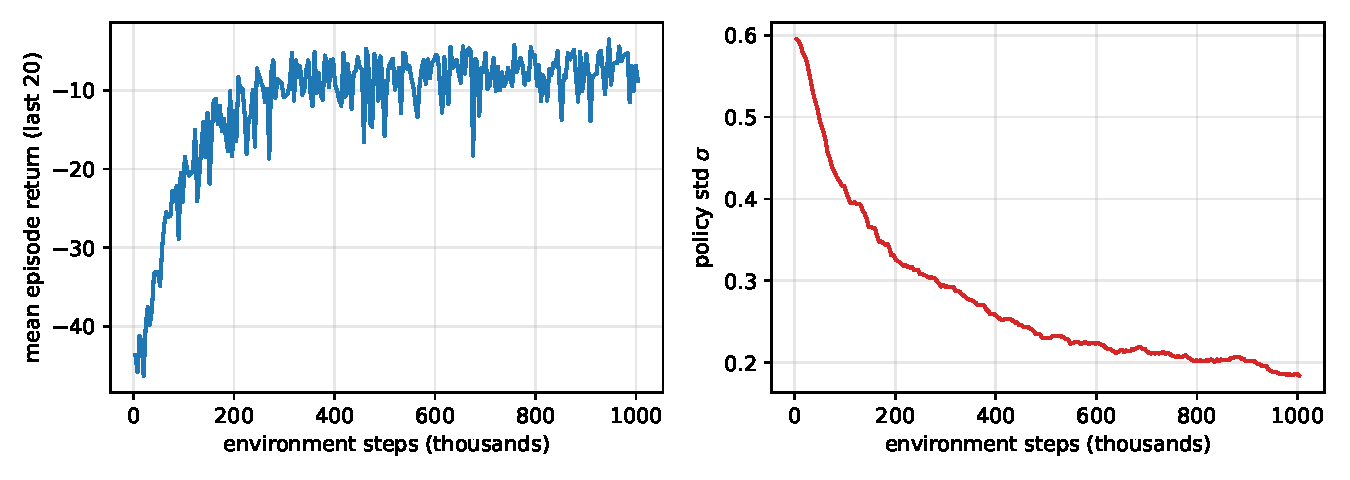
\includegraphics[width=0.95\textwidth]{figures/cascade_learning_curve.pdf}
\caption{Cascade training: mean return of the last 20 episodes (left) and
the mean policy standard deviation (right).}
\label{fig:cascade_learning}
\end{figure}

\subsection{Results}
All policies are evaluated on the same 30 held-out seasons (seeds
$10{,}000$--$10{,}029$). The tuned thresholds are
$\eta_A=0.2$, $\eta_B=0.5$.

\begin{table}[h]
\centering
\small
\begin{tabular}{lrrrrrrr}
\toprule
Policy & Return & Supply & Flood & Spill & Terminal & Deficit [\%] & Flood days \\
\midrule
Supply only & $-38.59\pm38.93$ & -1.12 & -14.23 & -22.74 & -0.50 & 3.1 & 9.4 \\
Rule (0.6, 0.5) & $-15.94\pm22.12$ & -1.18 & -7.41 & -6.64 & -0.71 & 2.8 & 8.2 \\
Tuned rule (0.2, 0.5) & $-14.07\pm19.26$ & -2.19 & -6.30 & -4.48 & -1.10 & 5.1 & 11.4 \\
PPO & $-12.27\pm17.30$ & -1.78 & -6.01 & -3.45 & -1.03 & 5.3 & 8.5 \\
\bottomrule
\end{tabular}

\caption{Cascade: mean over 30 test seasons, with columns as in
Table~\ref{tab:results}.}
\label{tab:cascade_results}
\end{table}

\begin{table}[h]
\centering
\begin{tabular}{lrrr}
\toprule
baseline & mean(PPO $-$ baseline) & std.\ error & PPO better in \\
\midrule
Supply only & $+26.32$ & 5.47 & 21/30 \\
Rule (0.6, 0.5) & $+3.67$ & 1.34 & 18/30 \\
Tuned rule (0.2, 0.5) & $+1.79$ & 0.67 & 22/30 \\
\bottomrule
\end{tabular}

\caption{Cascade: paired differences in season return, PPO minus
baseline.}
\label{tab:cascade_paired}
\end{table}

\paragraph{Headline.} In the cascade, PPO beats every baseline, including
the rule with tuned thresholds. Against the tuned rule, the season-by-season
difference is $+1.79\pm0.67$: about 2.7 standard errors, with PPO better in
22 of the 30 test seasons (Table~\ref{tab:cascade_paired}). In the
single-reservoir problem the same comparison was a statistical tie. The
extra difficulty of coordinating two reservoirs around an uncontrolled
tributary is what lets the learned policy pull ahead. The size of the gain
over the tuned rule is modest (about 13\% of its penalty), but it is
consistent.

\paragraph{Where the gain comes from.} Table~\ref{tab:cascade_results}
splits the return into its parts. Compared with the tuned rule, PPO
spills 23\% less water (13{,}800 versus 17{,}900~m$^3$ per season), floods
the river on fewer days (8.5 versus 11.4), and has a slightly smaller
supply penalty with the same total shortfall ($\approx5\%$ of demand). The
three trajectory figures show the mechanisms:
\begin{itemize}
\item \textbf{Hedging in droughts (Figure~\ref{fig:cascade_traj_med}).}
In this median season a long dry spell empties both reservoirs under every
policy. The rules deliver the full demand until the water runs out and
then deliver almost nothing for about 20 days. PPO starts delivering
somewhat less than demand around day 15, \emph{before} the reservoirs are
empty, and stretches its storage further. Because the supply penalty is
\emph{squared}, many small shortfalls cost less than a few large ones:
spreading a 1{,}000~m$^3$/d deficit over twice as many days at half the
size halves its penalty. This is the classic \emph{hedging rule} of
reservoir operation theory. The agent was never told about it; it
discovered it from the shape of the reward.
\item \textbf{Anticipating storms (Figure~\ref{fig:cascade_traj_best}).}
In this storm-rich season PPO raises releases ahead of forecast storms, up
to and slightly above $\Qsafe$, and keeps more room in B, so the storms
around days 40--47 cause far less spill than under the rules.
\item \textbf{Where it loses (Figure~\ref{fig:cascade_traj_worst}).} In
the season where PPO does worst relative to the tuned rule, a cluster of
storms arrives at the very end of the season. The tuned rule happened to
be holding A very low (its 20\% threshold) and absorbed more of it. PPO,
which also weighs the end-of-season storage term, was fuller and spilled
more. A learned policy is better \emph{on average}, not in every season.
\end{itemize}

\paragraph{The rule baselines.} The threshold map
(Figure~\ref{fig:cascade_tuning}) shows the logic of the best rule: keep
the large upstream reservoir low ($\eta_A=0.2$) and the small downstream
one at half ($\eta_B=0.5$), so that A's slow, large storm volumes have room
while B buffers the fast local response. Even tuned, the rule cannot
\emph{change} these targets with the forecast or the season, and that
flexibility is what PPO adds. ``Supply only'', which never releases for
flood space, shows how much is at stake: it spills about 91{,}000~m$^3$ per
season and scores $-38.6$.

\paragraph{Lessons for applying RL.}
\begin{enumerate}\itemsep1pt
\item RL helps most where simple rules are structurally limited: several
interacting storages, uncontrolled inflows and forecasts. For one
reservoir, a well-tuned rule was as good.
\item The reward shapes the behavior. The hedging seen here follows from
the squared deficit penalty, and a linear penalty would not produce it.
\item Fair comparison requires tuned baselines, identical test seasons and
paired statistics. Against the untuned rule the gain would have looked
twice as large ($+3.7$).
\end{enumerate}


\begin{figure}[h]
\centering
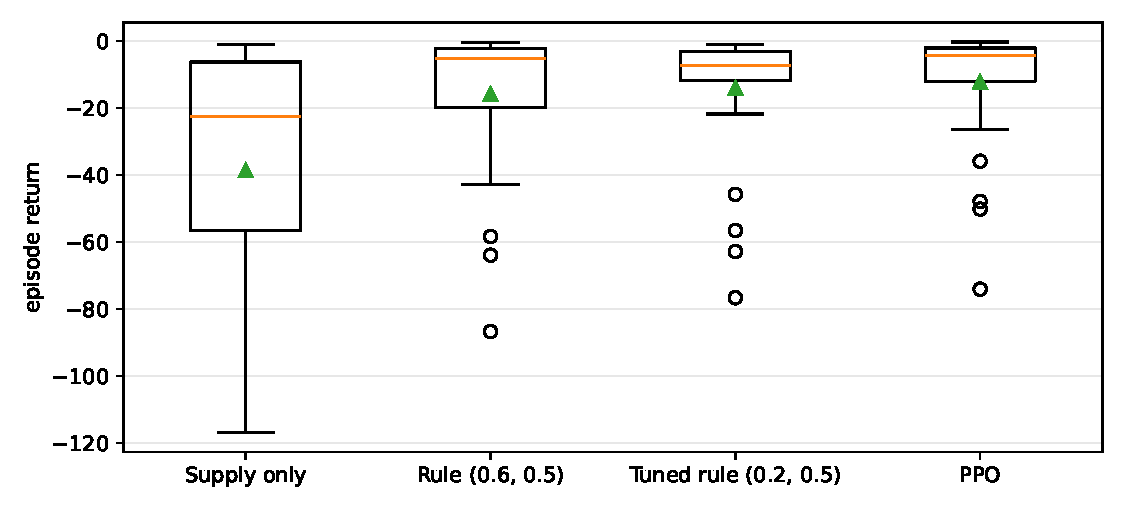
\includegraphics[width=0.7\textwidth]{figures/cascade_return_boxplot.pdf}
\caption{Cascade: distribution of test-season returns.}
\end{figure}

\begin{figure}[p]
\centering
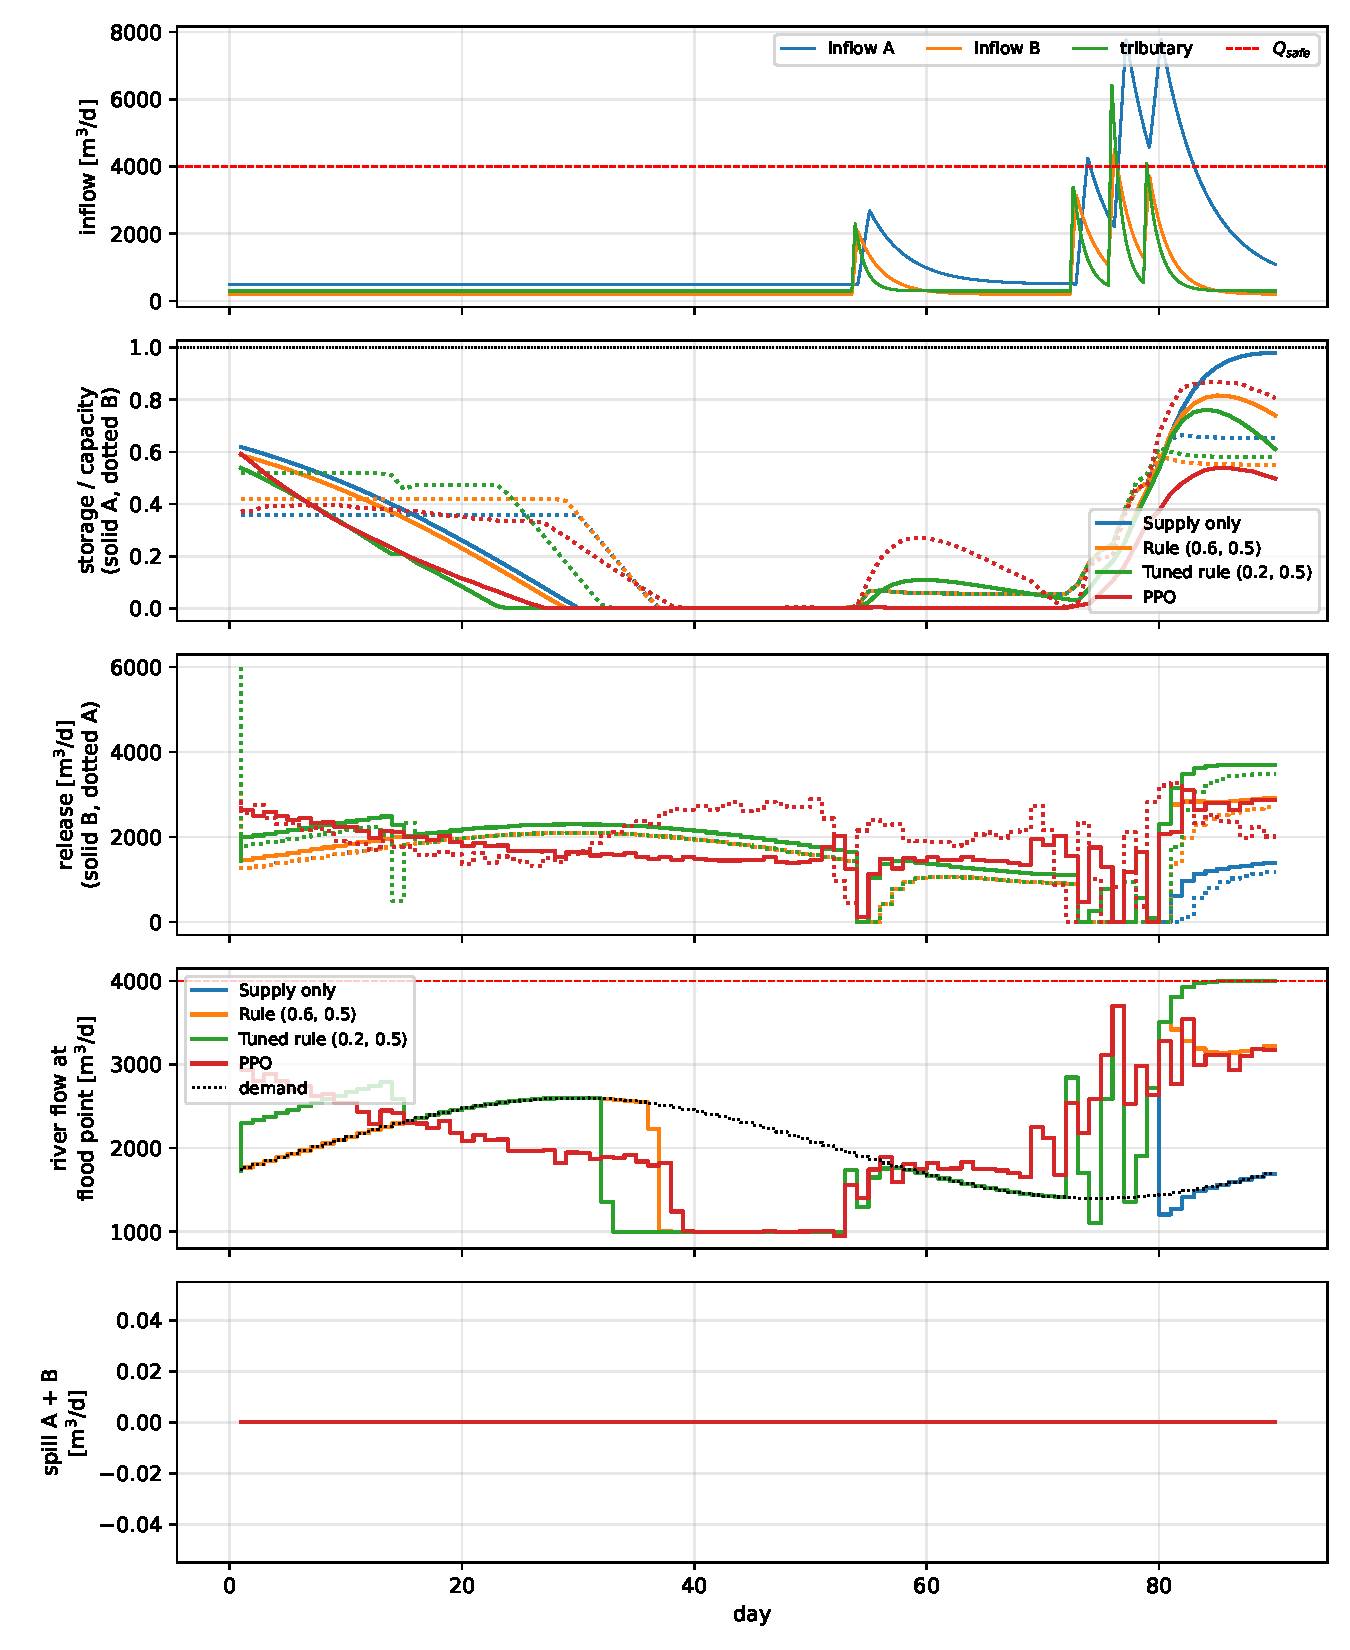
\includegraphics[width=0.92\textwidth]{figures/cascade_trajectory_median.pdf}
\caption{Cascade test season with the median PPO-vs-tuned-rule difference.
From top: the three inflows; storages (solid A, dotted B); releases (solid
B, dotted A); river flow at the flood point with demand (dotted) and
$\Qsafe$ (dashed); total spill.}
\label{fig:cascade_traj_med}
\end{figure}

\begin{figure}[p]
\centering
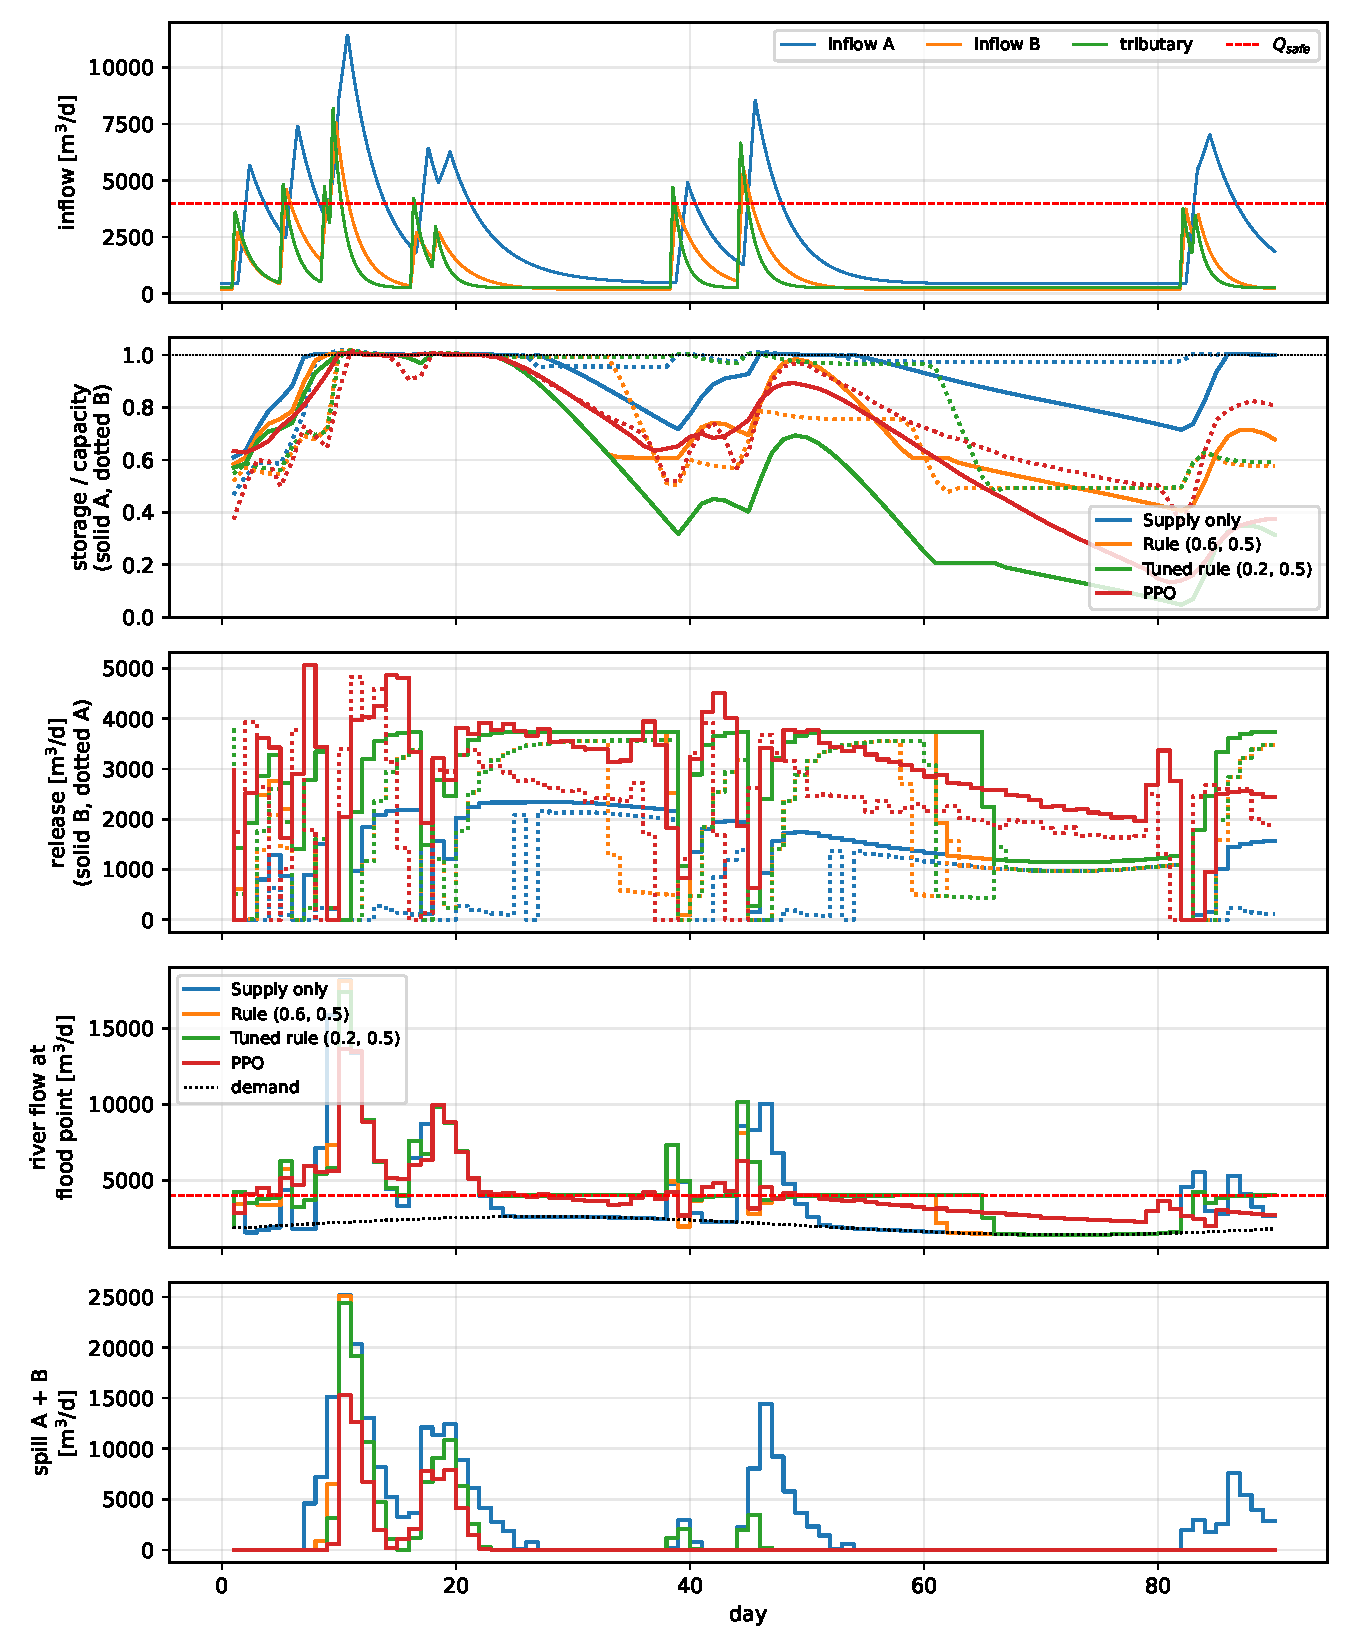
\includegraphics[width=0.92\textwidth]{figures/cascade_trajectory_best_gain.pdf}
\caption{Cascade test season with the largest PPO gain over the tuned rule.}
\label{fig:cascade_traj_best}
\end{figure}

\begin{figure}[p]
\centering
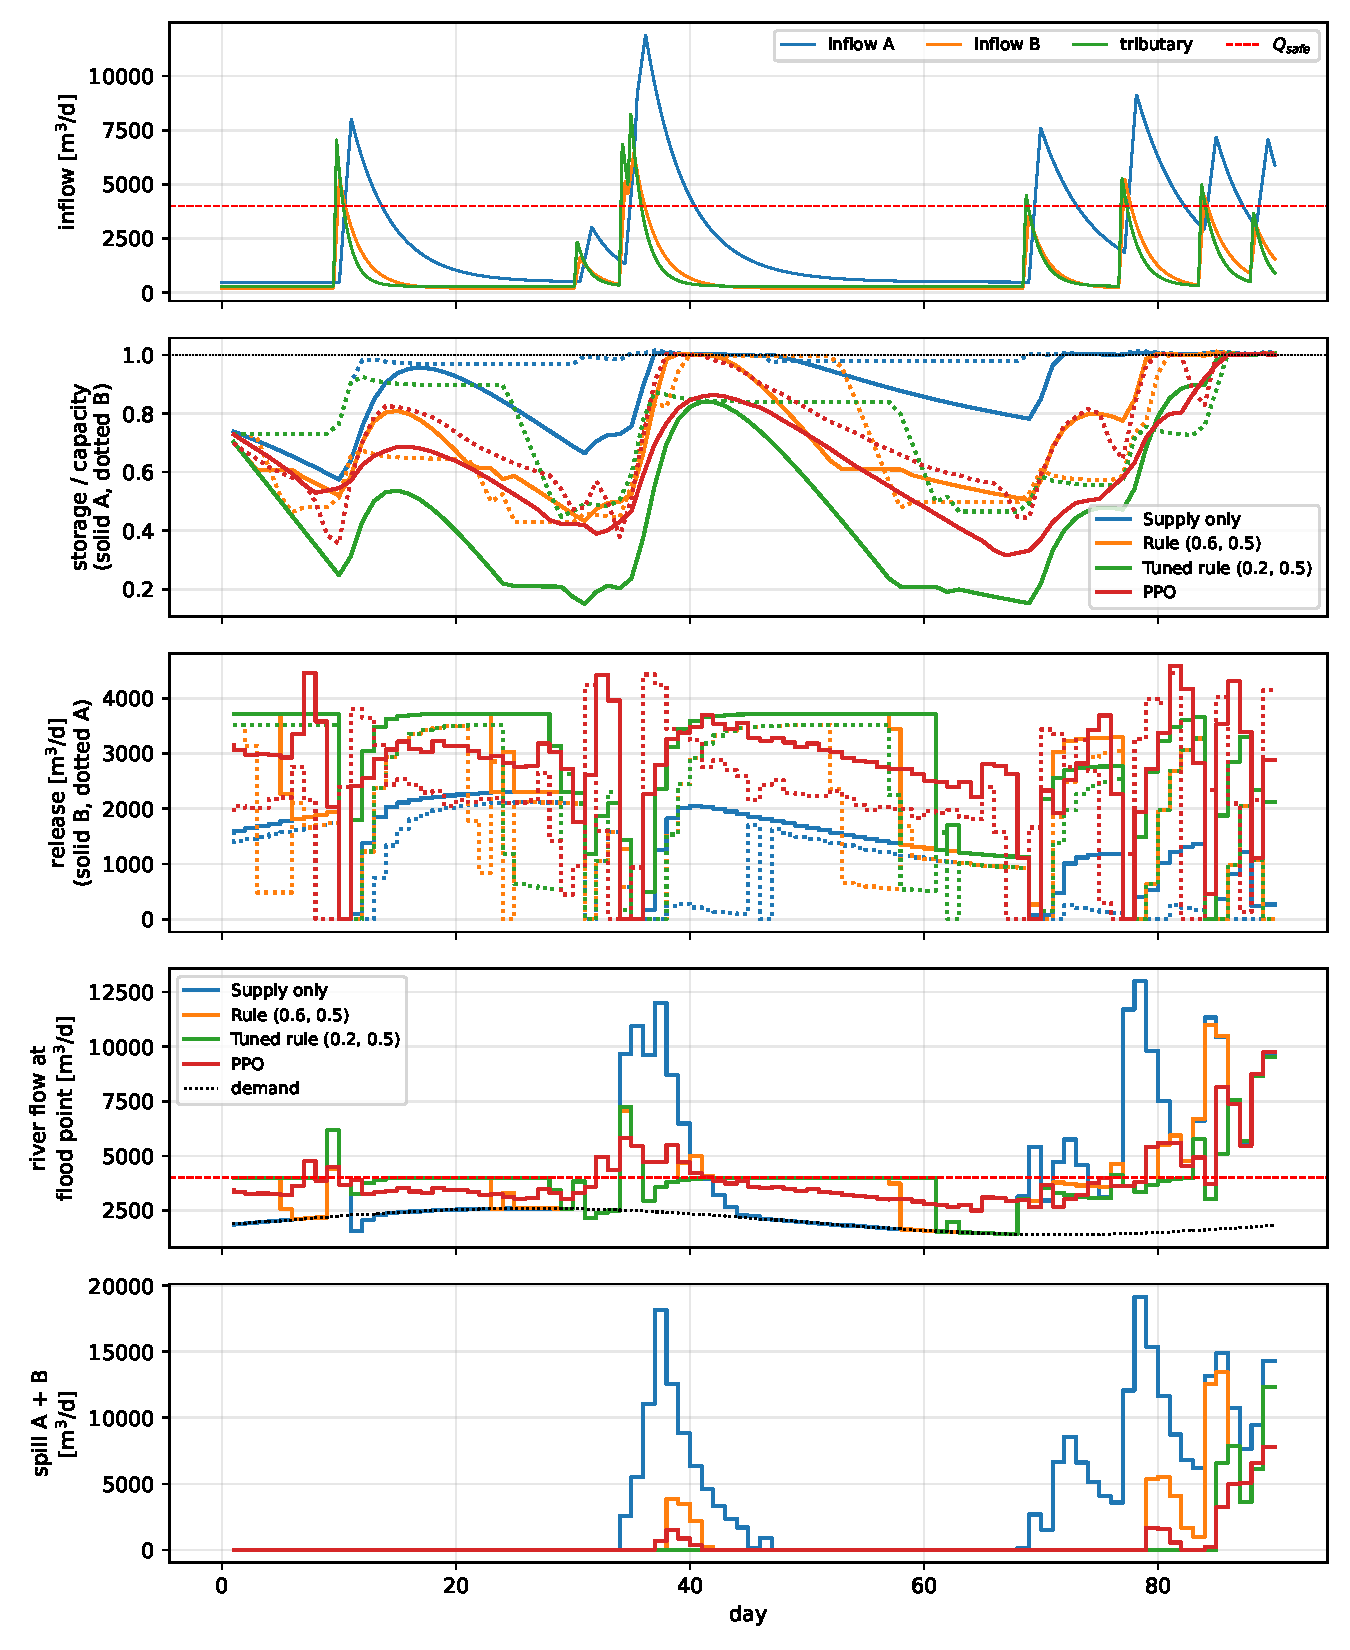
\includegraphics[width=0.92\textwidth]{figures/cascade_trajectory_worst.pdf}
\caption{Cascade test season where PPO does worst relative to the tuned rule.}
\label{fig:cascade_traj_worst}
\end{figure}
